\documentclass[a4wide]{report}

\usepackage{amsmath}
\usepackage[a4paper, total={7in, 10.2in}]{geometry}
\usepackage{graphicx}
\usepackage[portuguese]{babel}
\usepackage[utf8]{inputenc}


\begin{document}

\noindent
{\bf Rafael V. Cacilhas  - Relatório 03 (\today)}

\vspace{0.5cm}

\section*{Exercício 1}


\subsection*{1 a) }
Temos que as equações  do circuito podem ser escritas na forma:
\begin{equation}
R.i = V
\end{equation}
onde R é uma matriz 3x3 e i e V são matrizes 1x3. Assim, a equação pode ser escrita como:

$\begin{bmatrix} R_{1,1}  & R_{1,2}	&	R_{1,3} \\ R_{2,1}  & R_{2,2}	&	R_{2,3} \\R_{3,1}  & R_{3,2}	&	R_{3,3} \\ \end{bmatrix} \times \left[ \begin{array}{c} i_1 \\ i_2 \\ i_3 \end{array}\right]  =  \left[ \begin{array}{c} V_0 \\ 0 \\ 0 \end{array} \right] $

\vspace{1em}
Esta equação deve ser igual ao sistema de equações obtidos pela Lei de Kirchhoff:

$\begin{cases} 
r_{s} i_1 + r_1 i_2 + r_2 i_3 = V_0 \\ 
-r_{x} i_1 + (r_1 + r_x + r_a )i_2 - r_a i_3 = 0 \\  
-r_{3} i_1 -r_a i_2 + (r_2 + r_3 + r_a ) i_3 = 0
\end{cases} $

\vspace{1em}

Efetuando a multiplicação das matrizes e igualando os índices que multiplicam a mesma corrente temos que:

$\begin{cases} 
R_{1,1} = r_s \\ 
R_{1,2} = r_1 \\  
R_{1,3} = r_2 \\
R_{2,1} = -r_x \\ 
R_{2,2} = r_1 + r_x + r_a \\  
R_{2,3} = -r_a \\
R_{3,1} = -r_3 \\ 
R_{3,2} = -r_a \\  
R_{3,3} = r_2 + r_3 + r_a
\end{cases} $



\subsection*{b)}



U = 
 $\begin{pmatrix}
  u_{1,1}  & u_{1,2}	&	u_{1,3} \\
  0  & u_{2,2}	&	u_{2,3} \\
  0  & 0	&	u_{3,3} \\
 \end{pmatrix}$
 						
 \vspace{1em}
 
L = 
 $\begin{pmatrix}
  l_{1,1}  & 0	&	0 \\
  l_{2,1}  & l_{2,2}	&	0 \\
  l_{3,1}  & l_{3,2}	&	l_{3,3} \\
\end{pmatrix}$
 \vspace{1em}
 
Utilizando o algoritmo da Ref. [1] obtemos imediatamente os $u_{1,j}$ :

$\begin{cases} 
u_{1,1} = R_{1,1} \\ 
u_{1,2} = R_{1,2} \\  
u_{1,3} = R_{1,3}
\end{cases} $
 \vspace{1em}  
 
Deles, calculamos facilmente os $l_{i,1}$ :

$\begin{cases} 
l_{1,1} = \frac{R_{1,1}}{R_{1,1}} \\ 
l_{2,1} = \frac{R_{2,1}}{R_{1,1}} \\  
l_{3,1} = \frac{R_{3,1}}{R_{1,1}}
\end{cases} $
 \vspace{1em}
 
Note que $l_{1,1} = 1$. De fato, veremos que todos os termos da diagonal de L $l_{j,j}$ são iguais a 1. Tendo os $u_{1,j}$ e $l_{i,1}$ agora podemos calcular os $u_{2,i}$:

$\begin{cases} 
u_{2,2} = R_{2,2} - l_{2,1}u_{1,2} = R_{2,2} - \frac{R_{2,1} R_{1,2}}{R_{1,1} }  \\  
u_{2,3} = R_{2,3} - l_{2,1}u_{1,3} = R_{2,3} - \frac{R_{3,1} R_{1,3}}{R_{1,1} } 
\end{cases} $
 \vspace{1em}
 
Com estes, calculamos os $l_{i,2}$: 

$\begin{cases} 
l_{2,2} = \frac{1}{u_{2,2}}(R_{2,2} - l_{2,1}u_{1,2}) = 1 \\  
l_{3,2} = \frac{1}{u_{2,2}}(R_{2,2} - l_{2,1}u_{1,2}) =  \frac{1}{u_{2,2}}(R_{3,2} - \frac{R_{3,1} R_{1,2}}{R_{1,1}})  
\end{cases} $
 \vspace{1em}

E por fim podemos calcular $u_{3,3}$ e $l_{3,3}$: 

$\begin{cases} 
u_{3,3} = R_{3,3}  - (l_{3,1}u_{1,3} + l_{3,2}u_{2,3}) = R_{3,3} - \left(	\frac{R_{3,1}R_{1,3} }{R_{1,1}} + 	\frac{1}{ u_{2,2} }\left( R_{3,2} - \frac{R_{3,1}R_{1,2}}{R_{1,1}}\right) \left( R_{2,3} - \frac{R_{2,1}R_{1,3}}{R_{1,1}}	\right) 			\right)		 \\  
l_{3,3} = \frac{1}{u_{3,3}}(R_{3,3} - l_{3,1}u_{1,3} -l_{3,2}u_{2,3} ) = 1  
\end{cases} $
 \vspace{1em}

Na ultima equação deixamos o termo $u_{2,2}$ para evitar complicar demais as equações e dificultar o entendimento. 

\subsection*{ c) }
Na figura \ref{ponte} está representado as correntes calculadas. O valor obtido, arredondado para a terceira casa decimal, foi:
$\begin{cases} 
i_1 =  12.014 mA \\  
i_2 = 6.865	mA  \\
i_3 = 6.933 mA
\end{cases} $

Os valores com uma maior precisão podem ser visto na saída de dados do programa na tela. Podemos calcular a corrente no amperímetro utilizando a Lei dos Nós no ponto A:

\begin{equation*}
\Sigma i = 0
\end{equation*}

\begin{equation*}
i_{2} - i_{3} + i_{a} = 0
\end{equation*}

Foi obtido o valor $i_{a} =68.659 \mu A $. Assim como no caso acima, caso seja necessario uma precisão maior basta conferir a saída de dados na tela. Como $i_{a} \neq 0$ temos que a ponte não está balanceada.

\begin{figure}[!htb]
\centering
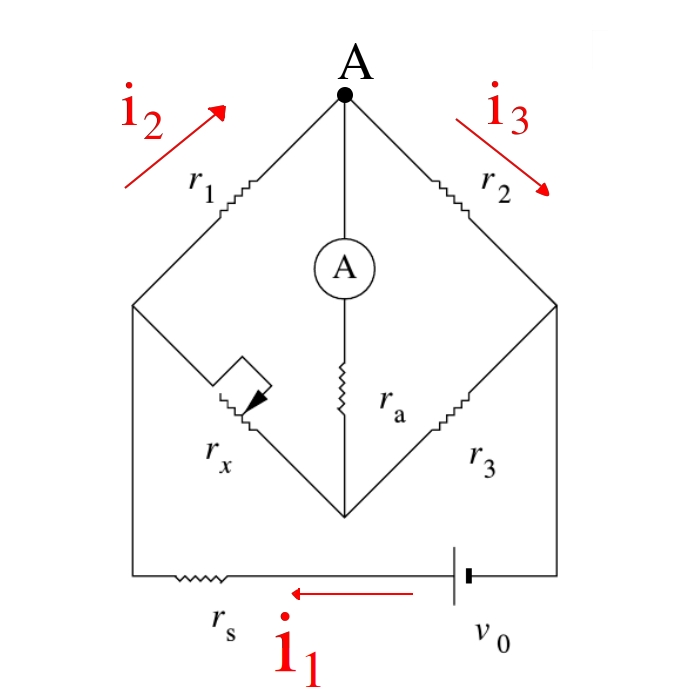
\includegraphics[width=0.447\textwidth]{ponte.jpg}
\caption{Ponte de Wheatstone com as correntes utilizadas.}
\label{ponte}
\end{figure}



\section*{Exercício 2}

\subsection*{a)}
O programa possui algum problema na decomposição LU, de modo que o produto LU não retorna exatamente x; há erros na terceira casa decimal, o que indica algum problema.

Não foi possível resolver o sistema nem encontrar o erro no algoritmo a tempo.







\section*{Exercício 3}
\subsection*{a)}
A lorentziana é dada pela fórmula:

\begin{equation}
P(\omega) = \frac{A}{\left[		(\omega - \omega_0)^2 + \Gamma				\right]}
\end{equation}
\label{p(w)}

Quando temos uma função $f(x) = [f_1(x_1,...,x_n),f_2(x_1,...,x_n),...,f_n(x_1,...,x_n)]$ temos que pela definição da matriz $\textbf{J}$:

$\vspace{5pt}$

J = $\begin{bmatrix}
    \frac{\partial f_1}{\partial x_1} & \frac{\partial f_1}{\partial x_2} &... & \frac{\partial f_1}{\partial x_n} \\
    \frac{\partial f_2}{\partial x_1} & \frac{\partial f_2}{\partial x_2} &... & \frac{\partial f_2}{\partial x_n}  \\
    ... &... &... &... &\\
    \frac{\partial f_n}{\partial x_1} & \frac{\partial f_n}{\partial x_2} &... & \frac{\partial f_n}{\partial x_n}
\end{bmatrix}$


\begin{equation*}
\frac{\partial P}{\partial A} = \frac{1}{\left[		(x - \omega_0)^2 + \Gamma				\right]}
\end{equation*}


\begin{equation*}
\frac{\partial P}{\partial \omega_{0}} = \frac{2A(x-\omega_0)}{\left[		(x - \omega_0)^2 + \Gamma				\right]^2}
\end{equation*}


\begin{equation*}
\frac{\partial P}{\partial \Gamma} = \frac{A}{\left[		(x - \omega_0)^2 + \Gamma				\right]^2}
\end{equation*}


Vamos definir duas variaveis auxiliares que simplificarão a escrita dessas variáveis:

$\begin{cases}
y_{sub} = \frac{1}{\left[		(x - \omega_0)^2 + \Gamma				\right]} \\  
x_{sub} = (x - \omega_0)
\end{cases} $

As derivadas segundas ficam:

\begin{equation*}
\frac{\partial^2 P}{\partial A^2} = 0
\end{equation*}

\begin{equation*}
\frac{\partial^2 P}{\partial A \partial \omega_0} = 2y_{sub}^2x_{sub}
\end{equation*}


\begin{equation*}
\frac{\partial^2 P}{\partial A \partial \Gamma} = y_{sub}^2
\end{equation*}



\begin{equation*}
\frac{\partial^2 P}{\partial \omega_{0}^2} = 2Ay_{sub}^2 \left[ 4x_{sub}y_{sub} + 1 \right]
\end{equation*}


\begin{equation*}
\frac{\partial^2 P}{\partial \omega_{0} \partial \Gamma} = -4Ax_{sub}y_{sub}^3
\end{equation*}


\begin{equation*}
\frac{\partial^2 P}{\partial \Gamma^2} = -2Ay_{sub}^3
\end{equation*}


As derivadas cruzadas são iguais independente da ordem.


Com isto, montamos J. No entanto não tive tempo de estudar e entender o resto do algoritmo, então paramos por aqui.


\subsection*{b)}

Os valores iniciais podem ser escolhidos analisando a equação e observando algumas características do grafico da função. Analisando a equação \ref{p(w)} vemos que o seu valor máximo (que ocorre em $\omega = \omega_0$ é $P(\omega) = \frac{A}{\Gamma}$. Assim sendo, sabemos que ao analisar o gráfico o ponto no eixo x onde ocorre o maior valor corresponde a $\omega_0$. O ponto y do maior valor corresponde a $\frac{A}{\Gamma}$. O parâmetro $\Gamma$ também determina a abertura da função. Um $\Gamma$ grande significa que a função é mais "achatada" que a mesma função com um $\Gamma$ menor. A análise, por exemplo, do ponto $\omega$ = 0 nos dá que $P(\omega) = \frac{A}{w_0^2 + \Gamma}$.




\section*{Exercício 4}
\subsection*{a)}
Dado a matriz H para calcularmos os autovalores temos que:

\begin{equation*}
\det(\textbf{H} -\lambda_n \textbf{I}) = 0
\end{equation*}

Ou seja:
\begin{equation}
(2 \omega_0^2 - \lambda)^3 -2(2 \omega_0^2 - \lambda)\omega_0^4 = 0
\end{equation}

Definindo a variavel auxilar $\alpha = (2 \omega_0^2 - \lambda)$, temos:

\begin{equation}
\alpha^3 - 2\alpha \omega_0^4  = 0
\end{equation}
\label{alpha}

\begin{equation*}
\alpha (\alpha^2 - 2\omega_0^4)  = 0
\end{equation*}

Cujas raízes são:
$\begin{cases} 
\alpha_1 =  0 \\  
\alpha_2 = + \sqrt{2}\omega^2  \\
\alpha_3 = - \sqrt{2}\omega^2
\end{cases} $

E temos que:

$\begin{cases} 
\lambda_1 =  \omega_0^2 (2-\sqrt{2}) \\  
\lambda_2 = 2\omega_0^2   \\
\lambda_3 =  \omega_0^2 (2+\sqrt{2})
\end{cases} $

\subsection*{b)}
Utilizamos o método de Newton-Raphson para descobrir as raízes da equação \ref{alpha}. Buscamos raízes no intervalo [0,2$\omega$]. Começamos com um "chute" inicial $x_0$ = 0 e utilizamos 200 $x_0$ igualmente espaçados no intervalo de interesse. Apenas duas raízes foram encontradas, o que era esperado visto que não é esperado que o computador ache as duas raízes da equação $\alpha^2 = 2\omega_0^4$. Fixamos que as duas primeiras raízes foram as encontradas pelo programa e que a terceira raíz foi a segunda raíz multiplicada por -1.

Tendo $\alpha$ basta aplicar $ \lambda = 2 \omega_0^2 - \alpha $. Os valores encontrados foram:
$\begin{cases} 
\lambda_1 =   9.3725822567939820\times10^{-2} \\  
\lambda_2 = 3.2000000000000006\times10^{-2}   \\
\lambda_3 =  5.4627417743206030\times10^{-1}
\end{cases} $

E os valores esperados são: 
$\begin{cases} 
\lambda_{1esperado} =   9.3725830020304796\times10^{-2} \\  
\lambda_{2esperado} = 3.2000000000000006\times10^{-2}   \\
\lambda_{3esperado} =  5.4627416997969525\times10^{-1}
\end{cases} $
        
Apresentando um erro na sétima casa decimal para $\lambda_1$ e $\lambda_3$ e uma precisão de 17 casas decimais para $\lambda_2$. A alta precisão para $\lambda_2$ se deve ao fato de que a raiz $\alpha = 0$ foi encontrada sem erro, com todas as casas decimais corretas.


\subsection*{c)}
O método da potência consiste em multiplicar sucessivas vezes a matriz \textbf{H} por um vetor inicial $\overrightarrow{u}_0$ arbitrário. Foi escolhido $\overrightarrow{u}_0 = (1,1,1)$ pela sua simplicidade.

Pelo método da potência temos que: 
\begin{equation}
\overrightarrow{u'}_{k+1} = \textbf{A}. \overrightarrow{u}_{k}
\end{equation}

Onde $\overrightarrow{u}_{k}$ é o vetor $\overrightarrow{u'}_{k}$ normalizado. Com isto, temos que :


\begin{equation}
\overrightarrow{u}_{k} = C \overrightarrow{u}_{3} 
\end{equation}

Ou seja, após sucessivas multiplicações por H o vetor escolhido passa a ser proporcional ao autovetor de maior autovalor associado. Em nosso programa, após 10 multiplicações sucessivas, obtemos que:

\begin{equation}
\overrightarrow{u}_{k} = (0.5,-0.71,0.5) 
\end{equation}

O que se encontra de acordo com o resultado esperado, visto que $\overrightarrow{u}_{3} = (1,-\sqrt{2},1)$. A saída do programa na tela apresenta uma maior precisão e divide o vetor $\overrightarrow{u}_{3}$ por 2 para uma comparação mais direta.


  
Um detalhe é que durante o estudo a tentativa de aplicar este algoritmo ao exemplo resolvido do livro não foi capaz de reproduzir os resultados deste. O exemplo na página 41 afirma que se encontra $\lambda_m = 4.907$, ao passo de que a equação 2.83 gera como resultado:
\begin{equation}
\lambda_m = x'_4.x_3 = 5.018806
\end{equation}



\end{document}
